\chapter{Introducción}\label{Chapter1} 
% chktex-file 8
% chktex-file 12
% chktex-file 13
% chktex-file 44

El avance en la capacidad de generar y almacenar datos ha llevado a la necesidad de transformar los datos crudos en conocimiento accionable que pueda optimizar la toma de decisiones en diversos sectores como salud, seguridad, educación, ciencia y negocios (BI). Para lograrlo, es fundamental desarrollar tecnologías que permitan ver y extraer información útil y conocimiento oculto en los datos, particularmente en grandes cantidades de datos textuales. Gestionar y analizar grandes cantidades de datos textuales puede ayudar a los usuarios a gestionar y hacer uso de este tipo de datos en todo tipo de aplicaciones.

\section{Datos textuales como \textit{Big Data}}
La gestión de texto de lenguaje natural, que abarca desde páginas web y redes sociales hasta literatura científica y documentos gubernamentales, se ha convertido en una prioridad debido a la explosión de datos en temas de todo tipo. Como un tipo especial de \textit{big data}, los datos textuales representan una gran oportunidad para el descubrimiento de conocimiento y optimización de decisiones en múltiples aplicaciones. Un ejemplo de ello son los datos textuales de opiniones (valoraciones de productos, foros, redes sociales, ...). \\

Dado el volumen creciente de datos textuales, es imposible para una persona consumir toda la información relevante en tiempo real, de modo que se requieren sistemas inteligentes de recuperación de información para facilitar el acceso rápido a los datos necesarios. El mundo genera entre 1 y 2 \textit{exabytes} de datos anualmente, de los cuales una gran cantidad es textual. \\

Atendiendo a la estructura de los datos, se pueden clasificar en dos tipos:
\begin{itemize}
\item Los datos estructurados, que cuentan con esquemas bien definidos, son manejados fácilmente por los ordenadores. 
\item Los datos no estructurados, como el texto, necesitan procesamiento computacional para interpretar su contenido, al tener una estructura menos explícita.
\end{itemize}

El procesamiento de lenguaje natural (NLP) aun no ha alcanzado un punto que permita al ordenador entender de forma precisa el texto. Generalmente se usan aproximaciones estadísticas y heurísticas para extraer información y analizar los datos textuales. El texto es de las fuentes de información más útiles ya que 
\begin{itemize}
\item Es la forma más natural de codificar el conocimiento humano. Por ejemplo, el conocimiento científico casi solo existe en literatura científica, los manuales técnicos dan explicaciones detalladas de como operar aparatos, ...
\item Es el tipo de información más frecuente.
\item Es la forma de información más expresiva.
\end{itemize}

\subsection{Recuperación y minería de texto}

\noindent Para gestionar y explotar grandes cantidades de datos textuales, se suele recurrir a dos técnicas. Se aplica la recuperación de textos sobre una gran cantidad de datos textuales para, sobre los datos relevantes extraídos, aplicar minería y obtener conocimiento que usar en distintas aplicaciones.

\subsubsection{Recuperación de texto (\textit{text retrieval})}

No se puede digerir toda la cantidad de información disponible, por lo que son necesarios sistemas inteligentes de recuperación de información para facilitar el acceso rápido a los datos necesarios. Para esto surgen los motores de búsqueda, útiles en cualquier contexto donde haya una gran cantidad de datos textuales, no solo en la \textit{web}. 

\subsubsection{Minería de texto (DM)}

Los datos textuales son ricos en contenido semántico. La minería de texto busca descubrir conocimiento valioso dentro del contenido textual, usando herramientas de \textit{software} inteligentes para descubrir patrones interesantes y opiniones que optimicen la toma de decisiones. El proceso de minería de datos puede describirse como minar los datos textuales para descubrir conocimiento útil. \\

La minería de datos aún no es tan madura como los motores de búsqueda, ya que el texto tiene una estructura menos explícita. El desarrollo de minería inteligente requiere que los ordenadores entiendan el contenido codificado en el texto. 

\subsection{Modos de acceso a la información: Pull vs Push}

En el modo \textit{pull}, el usuario toma la iniciativa de buscar información en el sistema, mientras que este último juega un papel pasivo y espera la petición del usuario. En las consultas, el usuario especifica la información necesaria y el sistema devuelve documentos que considera relevantes. \\

En el modo \textit{push}, el sistema recomienda información anticipando las preferencias y necesidades de información del usuario. Suele funcionar bien cuando el usuario tiene una necesidad de información relativamente estable, como un \textit{hobby}. Aquí, el sistema puede conocer las preferencias e intereses del usuario con adelanto. \\

En la navegación, el usuario se mueve por estructuras que enlazan elementos de información y alcanza información relevante progresivamente. La navegación y las consultas se alternan de forma natural. 

\section{Sistemas de Información Textual (TIS)}

Estos sistemas buscan dar acceso a la información: conectan la información adecuada con el usuario adecuado en el momento adecuado. Ejemplos clásicos son:
\begin{itemize}
\item Motores de búsqueda: permiten al usuario acceder a información textual a través de consultas.
\item Sistemas de recomendación: pueden sugerir información relevante al usuario de forma proactiva. 
\end{itemize}

Se debe realizar un análisis de texto suficiente como para emparejar la información relevante con la información que necesita el usuario. Los elementos de información originales se muestran en su forma original, aunque en ocasiones se muestra a través de resúmenes dinámicos que dependen de la búsqueda del usuario (\textit{snippets}).

\subsection{Análisis del texto}

Un análisis del texto permite adquirir el conocimiento útil codificado en los datos textuales, el cuál no es fácil de obtener sin sintetizar y analizar una gran cantidad de los datos. Por ejemplo, un motor de búsqueda simplemente devuelve las valoraciones relevantes de un producto, mientras que un motor de análisis extrae las opiniones positivas y negativas y compara opiniones de multitud de productos. \\

Los sistemas de información textual anotan una colección de documentos textuales con estructuras (tópicos) relevantes. Estas estructuras añadidas permiten al usuario buscar con restricciones sobre las mismas o navegar siguiéndolas. \\

A diferencia del DM, que se mueve bajo la premisa de descubrir y extraer patrones interesantes en los datos textuales, el NLP se mueve bajo la premisa de entender del texto de lenguaje natural de forma parcial, convertirlo en una forma de representación de conocimiento y hacer inferencia basándose en el conocimiento extraido. 

\subsection{Sistemas de información textual}
Los TIS integran servicios de análisis de contenido basados en procesamiento de lenguaje natural (NLP) para transformar datos textuales crudos en representaciones más significativas, apoyando así la recuperación, categorización y organización de información. Se suele combinar el aprendizaje automático estadístico con conocimiento linguístico limitado. Las técnicas poco profundas son robustas, pero un análisis semántico profundo solo es factible en dominios específicos. \\

Algunas habilidades, como la de resumir documentos, requieren técnicas de NLP más profundas que otras, como una simple búsqueda. Sin embargo, la mayorías de TIS usan técnicas poco profundas, como bolsas de palabras. 

\begin{figure}[h]
\centering
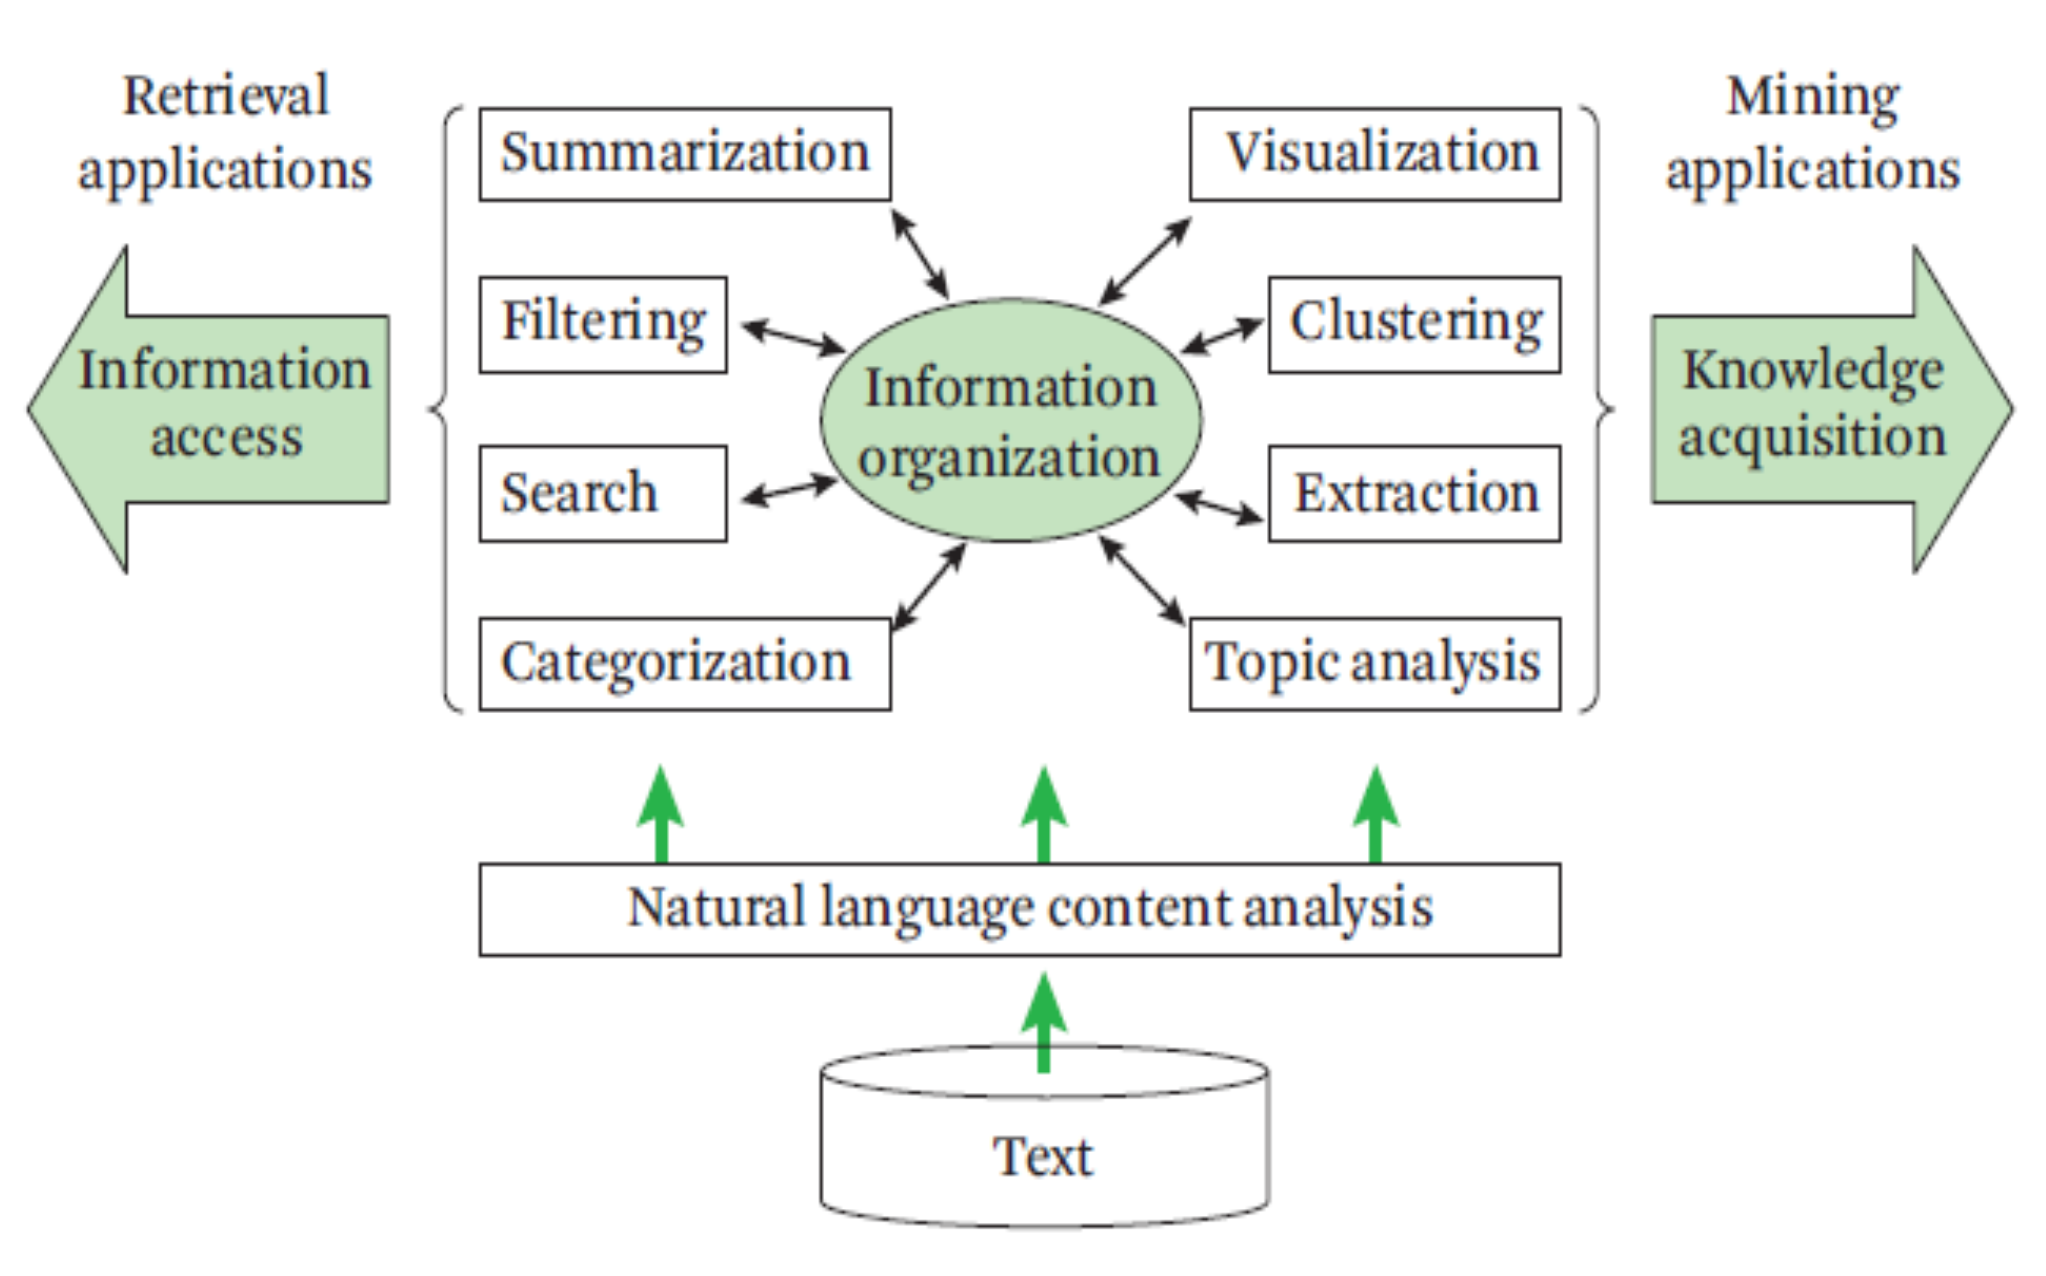
\includegraphics[width=0.5\textwidth]{fotos/1.png}
\caption{Esquema conceptual de un TIS}
\label{fig:1}
\end{figure}

\noindent Existen varias formas de organizar la información en un TIS:

\begin{itemize}
    \item \textbf{Búsqueda}: toma una consulta del usuario y devuelve documentos relevantes.
    \item \textbf{Filtrado y Recomendación}: monitoriza el flujo de datos, selecciona los ítems relevantes para los intereses del usuario y luego recomienda los items relevantes (o filtra los no relevantes). Un sistema de recomendación tiene como objetivo recomendar información relevante al usuario, mientras que un sistema de filtrado tiene como objetivo filtrar la información no relevante, permitiendo que el usuario mantenga solo los \textit{items} relevantes.
    \item \textbf{Categorización}: clasifica un objeto textual en una o varias categorías predefinidas. Puede anotar los objetos con todo tipo de categorías significativas, enriqueciendo la representación de los datos textuales. En este caso hay dos tipos de errores, los falsos positivos y los falsos negativos; hay que ver que métrica de rendimiento se le da al clasificador, dando más o menos \textit{penalty} a un error concreto. Estos sistemas son tradicionales, y se usaban para, por ejemplo, clasificar correos electrónicos como \textit{spam}.
    \item \textbf{Resumen}: toma uno o varios documentos de texto y genera un resumen conciso de los contenidos esenciales. Reduce el esfuerzo humano de digerir grandes cantidades de información textual.
    \item \textbf{Análisis de temáticas}: toma una serie de documentos y extrae y analiza los temas en ellos. Los temas aydan a digerir la información y permiten navegar por el texto de forma cómoda. Se puede combinar con datos no textuales, como tiempo, localización u otros metadatos. De este modo, es capaz de generar patrones de interés (tendencias temporales de temáticas, distribución espacio-temporal del tópicos, etc). Es tecnología no supervisada, por lo que los temas no están predefinidos, los da el propio algoritmo.
    \item \textbf{Extracción de información}: Extrae entidades y relaciones de entidades con otras áreas de conocimiento. 
    \item \textbf{Clustering}: descubre grupos de objetos textuales similares (términos, oraciones, documentos, etc). Ayuda a los usuarios a explorar un espacio de la información, y es útil para descrubrir \textit{outliers}. 
    \item \textbf{Visualización}: permite representar visualmente patrones en los datos textuales.
\end{itemize}